\documentclass[a4paper,oneside,12pt]{article}
\usepackage{polyglossia}
\usepackage{microtype}
\setdefaultlanguage{english}
%\setotherlanguages{english}
\usepackage{fontspec}
\usepackage{amsmath}
\usepackage{amssymb}
\usepackage{amsfonts}
\usepackage{mathtools}
\usepackage{xltxtra}
\usepackage{xunicode}
\defaultfontfeatures{Mapping=tex-text}

\sloppy

%\usepackage[utf8]{inputenc}
%\usepackage[english,russian]{babel}
\usepackage{fancyhdr}
\usepackage[colorlinks=true,hidelinks]{hyperref}
\usepackage{ushort}
\usepackage{textcase}
\usepackage{tabularx}
\usepackage{colortbl}
\usepackage{graphicx}
\usepackage[x11names]{xcolor}
\usepackage[left=20mm,right=20mm,top=22mm,bottom=22mm]{geometry}
\setlength{\parindent}{0em}
\definecolor{dark}{RGB}{0,0,0}

\pagestyle{fancy}
\fancyhead{}
\fancyfoot{}
\fancyfoot[RO,RE] {\thepage}
\renewcommand{\headrulewidth}{0pt}
\renewcommand{\footrulewidth}{0pt}

\def\labelitemi  { \raisebox{0.1em} {$\scriptscriptstyle \blacksquare$} }
\def\labelitemii { \raisebox{0.1em} {$\scriptscriptstyle \Box        $} }
%\def\labelitemiii{ \raisebox{0.1em} {$\scriptscriptstyle $} }

\newcommand{\cvpart}[1]{%
\vspace{-0.9em}%
\section*{\Large\bfseries\MakeTextUppercase{#1}}%
\vspace{-1.7em}%
\rule{\linewidth}{0.3em}\\[-0.8em]%
}


\begin{document}

\begin{centering}
\begin{minipage}{0.70\linewidth}%
\vspace{-1.5em}{\Huge\bfseries Ivan Baravy}

~\\[-1.5em]

\hspace{1.9em}\begin{tabularx}{\linewidth}{ll}
{\it E-mail:}		& ivan\_baravy@apmath.spbu.ru\\
{\it Phone:}	        & +7\,(950)\,026-49-36 (mobile)\\
~\\[-1.0em]
{\it Address:}	    & ul.\,Botanicheskaya, 64/3, ap.\,310a,\\
                    & Stary Petergof, St.\,Petersburg,\\
                    & 198504, Russia\\
~\\[-1.0em]
{\it Date of birth:}	& 4 May 1991\\
{\it Marital status:}& single\\
{\it Citizenship:}   & Republic of Belarus\\
{\it Languages spoken:}& English (advanced), German (basic),\\
		       &Russian (expert), Belarusian (native)\\
\end{tabularx}
\end{minipage}
\begin{minipage}{0.23\linewidth}%
\begin{flushright}
%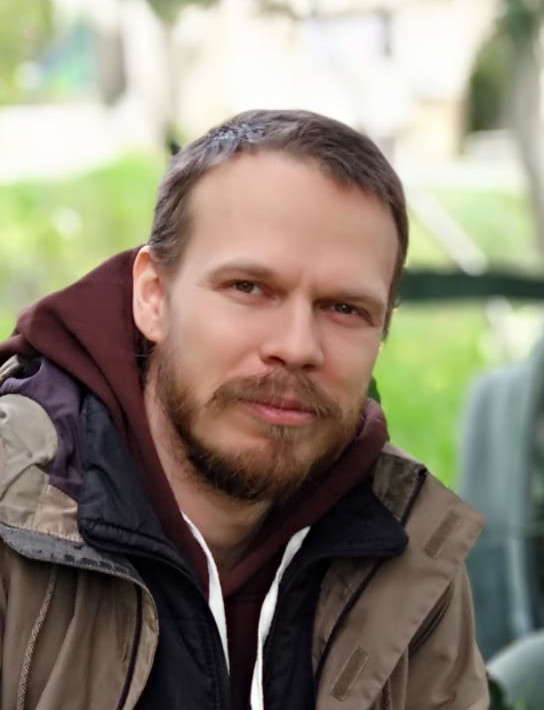
\includegraphics[width=35mm]{me.jpg}
{%
\setlength{\fboxsep}{0pt}%
\setlength{\fboxrule}{0pt}%
\fbox{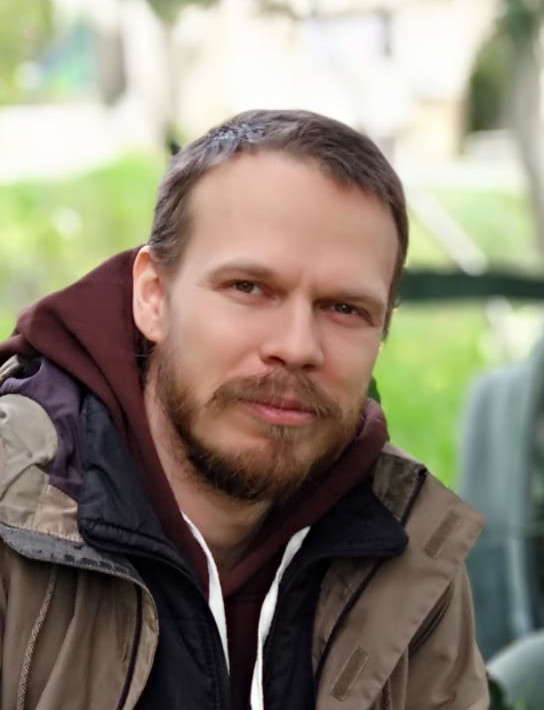
\includegraphics[width=35mm]{me.jpg}}
}%
\end{flushright}
\end{minipage}
\end{centering}
~\\[1.5em]


\cvpart{Summary}
\begin{itemize}
\item 3 years of experience in UNIX programming environment (GNU/Linux, OpenBSD).
\item Strong knowledge of C language (ANSI~C, C99) and GNU toolchain.
\item Experience in low--level / system programming (x86, x86\_64, arm, e2k).
\item Experience in developing real-time applications under RTOS (ARINC--429, OS2000).
\item Experience in development of cross-platform applications (POSIX, libc).
\item Development of multithreaded applications (fork, libpthread, OpenMP).
\item Deep knowledge of i686 and x86\_64 architectures and assembly languages.
\item Experience in Linux modules development.
%\item Version control systems (git, subversion).
\item Perl and shell scripting, software integration.
\item Digital signal processing.
\item Discrete math and algorithm design.
%\item Parallelization and vectorization techniques.
\item Experience in project management.
\end{itemize}


\cvpart{Technical skills}
\begin{description}
\item[Operating systems:] Linux 2.6.x/3.x, OpenBSD 4.x/5.x, FreeDOS, KolibriOS, Windows NT4/XP.
\item[Programming languages:] C (ANSI~C, C99) / C++, x86 and x86\_64 assembly (i386-i686, SIMD: MMX, SSE\{2,3,4\}, AVX), Perl, sh and bash scripting.
\item[Developer tools:] GNU toolchain (GCC, gdb, make, binutils), valgrind, git, subversion, (g)vim, qemu/kvm, doxygen.
\item[Standards, technologies, libraries:] POSIX, ARINC--429, OpenMP, MPI, RapidIO, milstd--1553b, rfc6919, libc/musl, libpthread, librt, libeml, libfftw, sqlite, libgmp, libxml2, libx11, libmagickwand, libimg, libcrash.
\item[Digital signal processing:] FFT/IFFT, DWT/IDWT, Z--transform, filtering, denoising, compression, color space transforms, image recognition.
\item[Cryptography:] symmetric and public-key cryptography, RSA, ElGamal, digital signature, cryptographic hash functions (sha1, sha2, sha3/keccak).
\item[Coding theory:] finite/Galois fields, error control coding, Hankel polynomials, Hamming codes, Reed--Solomon codes, wavelet codes, non-cryptographic hash functions (crc32, md4, md5, murmur, siphash), perfect hashing, Huffman coding, Lempel--Ziv coding, deflate.
\item[Other skills:] Packaging (Debian, Arch), markdown, LaTeX.
\end{description}



\cvpart{Employment}

\begin{tabularx}{\linewidth}{lX}
2012~-- to present:& CSPA Leninetz, Software Engineer.\\
2014~-- to present:& Saint Petersburg State University, Research Engineer.\\
2013~-- 2014:& Saint Petersburg State University, Laboratory Assistant.
\end{tabularx}


\cvpart{Education and Science}

\begin{tabularx}{\linewidth}{rX}
2014~-- to present:& Saint Petersburg State University (PhD student)\\
           faculty:& Applied Mathematics and Control Processes\\
        department:& Control of Medical and Biological Systems\\
                   & \\
      2009~-- 2014:& Saint Petersburg State University (graduate)\\
           faculty:& Applied Mathematics and Control Processes\\
        department:& Mathematical Modelling and Multiprocessor Systems\\
            Thesis:& 'Wavelets in Error Control Coding: Analysis of Linear Codes'\\
            Degree:& Specialist's degree in Applied Mathematics and Information Technology
\end{tabularx}

~\\

List of publications:
\begin{itemize}

\item Baravy I. Efficient Interpolation over Infinite and Finite Fields via Hankel Polynomials~// 19th International
Conference Mathematical Modelling and Analysis, Abstracts. Druskininkai, Lithuania. 2014.~--- P. 9

\item Baravy I. Wavelets in Digital Audio Processing: Beethoven's Sonatas Clustering~// Proceedings of the XLIV International Conference
Control Processes and Stability. St.Petersburg, Russia. 2013.~--- P. 513\,--\,516

\item Uteshev A.Yu., Baravy I. Inversion in finite fields with the aid of Hankel polynomials~// International Conference
on Computer Science and Information Technologies. Yerevan, Armenia. 2013.~--- P. 124\,--\,127
\end{itemize}


\cvpart{Scholarships and Grants}

\begin{tabularx}{\linewidth}{rX}
Sep 2013~-- Jun 2014:& St.\,Petersburg State University research grant 9.38.674.2013 for developing generic interpolation algorithm over infinite and finite fields via Hankel matrices and polynomials; attending MMA\,2014 con\-fe\-ren\-ce~(Druskininkai, Lithuania) with oral presentation.
\end{tabularx}

\begin{tabularx}{\linewidth}{rX}
Jan 2013~-- Sep 2013:& Scholarship from \href{http://www.raidixstorage.com}{RAIDIX}\footnote{\url{http://www.raidixstorage.com}} for research in coding theory and application of Hankel polynomials to the inversion problem in finite fields; participation in CSIT\,2013 conference~(Yerevan, Armenia) and publication in a journal indexed by SCOPUS.
\end{tabularx}


\cvpart{Participation in Open Source Projects}
\begin{itemize}
\item Conferences, unconferences and contests
\begin{itemize}
\item 2014~--- Google Reunion. San Jose, California, USA.\\
{\color{gray}\small\url{https://sites.google.com/site/gsocmentorsummitstudentreunion/}}\\
Role: Delegate.
\item 2014~--- Google Summer of Code.\\
{\color{gray}\small\url{https://www.google-melange.com/gsoc/homepage/google/gsoc2014}}\\
Role: Mentor.\\
Goal: Supervise accepted student, manage his project.\\
Result: Student's code merged into upstream.
%\item 2014~--- VALS Semester of Code. Member.
\item 2013~--- KolibriOS Summer of Code.\\
{\color{gray}\small\url{http://wiki.kolibrios.org/wiki/KolibriOS_Summer_of_Code_2013}}\\
Role: Student.\\
Goal: Implement XFS filesystem support.\\
Result: Code merged into upstream.
\item 2013~--- Intel Accelerate Your Code, Summer.\\
{\color{gray}\small\url{http://www.intel-software-academic-program.com/contests/ayc/2013-summer/}}\\
Role: Student.\\
Goal: Parallelize and vectorize image recognition code.\\
Result: Winner (Ultrabook).
\end{itemize}
\item libcrash~--- multiplatform library of cryptographic hash functions
\begin{itemize}
\item Architecture design and implementation.
\item Implementing hash functions: md4, md5, sha1, sha2~(sha224, sha256, sha384, sha512), sha3/keccak~(sha3-224, sha3-256, sha3-384, sha3-512).
\item Assembly programming and optimizations for i686, x86\_64.
\end{itemize}

\item \href{http://websvn.kolibrios.org/listing.php?repname=Kolibri+OS}{KolibriOS~--- Operating System, i586+}
\begin{itemize}
\item \href{http://websvn.kolibrios.org/listing.php?repname=Kolibri+OS&path=%2Fkernel%2Ftrunk%2Ffs%2F&#a0aa5cede7308db82d4bae78266ed8462}{kernel}
\begin{itemize}
\item XFS file system support (read only).
\item Vulnerability analysis.
\item Bugfixing.
\end{itemize}
\item \href{http://websvn.kolibrios.org/listing.php?repname=Kolibri+OS&path=%2Fprograms%2Fdevelop%2Fasciivju%2Ftrunk%2F&#a5da69869b5757c5b71158a900f51c0c3}{ASCIIVju~--- developer utility for checking keyboard scancodes}
\begin{itemize}
\item Disassembling.
\end{itemize}
\item \href{http://websvn.kolibrios.org/listing.php?repname=Kolibri+OS&path=%2Fprograms%2Fdevelop%2Flibraries%2Flibs-dev%2Flibimg%2F&#ac73184f3b97abb1a3031cce2f0fae471}{libimg~--- system library to decode, encode, scale and convert raster images}
\begin{itemize}
\item Digital image processing: scaling, converting, transforming.
\item SIMD instructions optimization (MMX, SSE).
\item Decoders for webp (LZ77, color cache), tiff (RLE, LZW), xcf, pnm, pcx and other raster formats.
\item Documentation.
\item Bugfixing.
\end{itemize}
\end{itemize}
\end{itemize}


\cvpart{Professional Experience}

{\bf
CSPA Leninetz, St.\,Petersburg, Russian Federation. Software Engineer. Full-time position.\\
July 2012~--- to present
}

\begin{itemize}
\item Algorithm design and implementation for processing signal of aircraft radar (digital signal processing, FFT/iFFT, algorithm design).
\item Real-time applications development for on-board control system (ARINC--429, milstd--1553b, RapidIO, OS2000, 0S3000).
\item Porting on-board control system code from MIPS64 to e2k (C, GNU toolchain).
\item Debugging and profiling of multithreaded applications~--- on-board control system (gdb, valgrind).
\item API design and writing documentation for interprocessor interaction framework (C99, doxygen).
\item Software integration~--- developing test stand for on-board system certification (C, shell).
\end{itemize}

~\\[-1em]

{\bf
Saint Petersburg State University, St.\,Petersburg, Russian Federation. Laboratory Assistant, Research Engineer. Part-time position.\\
March 2013~--- to present
}

\begin{itemize}
\item Scientific research in finite fields and coding theory at the Faculty of Applied Mathematics and Control Processes.
\item Numerical simulation of fluid flow and thermodynamic processes (turbulence) in mathematics software Sage~(Maxima, NumPy, matplotlib).
\item Participation with oral presentations in international conferences on applied mathematics.
\item Development and implementation of distributed versions for common data processing algorithms in NUMA environments using MPI and OpenMP.
\end{itemize}

\end{document}
% link to libcrash
% project/role in professional experience
% separate laboratory assistant and research engineer
